%卒論中間審査用研究概要テンプレート ver. 1.1

\documentclass[uplatex,twocolumn]{jsarticle}
\usepackage[top=22mm,bottom=22mm,left=20mm,right=20mm]{geometry}
\setlength{\columnsep}{15mm}
\usepackage[T1]{fontenc}
\usepackage{txfonts}
\usepackage{wrapfig}
\usepackage[expert,deluxe]{otf}
\usepackage[dvipdfmx,hiresbb]{graphicx}
\usepackage[dvipdfmx]{hyperref}
\usepackage{pxjahyper}
\usepackage{secdot}

\makeatletter
\renewcommand{\section}{%
  \@startsection{section}{1}{\z@}%
  {0.6\Cvs}{0.4\Cvs}%
  {\normalfont\normalsize\raggedright}}
\renewcommand{\subsection}{\@startsection{subsection}{2}{\z@}%
  {\z@}{\z@}%
  {\normalfont\normalsize}}
\renewcommand{\subsubsection}{\@startsection{subsubsection}{3}{\z@}%
  {\z@}{\z@}%
  {\normalfont\normalsize}}
\makeatother
%ここから上を編集する必要はない.





%タイトルと学生番号,名前だけ編集すること
\title{\vspace{-5mm}\fontsize{14pt}{0pt}\selectfont GitHubを用いた開発フローの判別分析}
\author{\normalsize プロジェクトマネジメントコース・ソフトウェア開発管理グループ 矢吹研究室 1242132 若月 純}
\date{}
\pagestyle{empty}
\begin{document}
\fontsize{10.5pt}{\baselineskip}\selectfont
\maketitle





%以下が本文
\section{研究の背景}

ソフトウェア開発では,GitHubを用いることが多い.GitHubは,バージョン管理システムに加え,branch,PullRequest,Issuesといった開発を補助する機能を提供するサービスである.
 
GitHubを使用する手順を開発フローと呼ぶ.現在わかっている開発フローの数は13個ある\cite{onodera2015}.開発フローの例を1つあげる.GitHub Flowは,作業をするbranchを作成し,完成したら統合する.というような開発フローである.この開発フローはとてもシンプルなため,開発フローを実施するまでの学習コストは,抑えられるが,開発規模が大きい場合,PullRequestがたまりやすく,コードレビューに時間がかかってしまうことがある\cite{okumura2013}.

このように開発フローは,メリット・デメリットがある.そのため,開発フローをプロジェクトの性質から選択する基準が必要である. 


\section{目的}

GitHubを用いたソフトウェア開発プロジェクトの性質において,適切な開発フローを選択できるようにするための基準を提供する.


\section{研究方法}

初めに,GitHub上のプロジェクトから,プロジェクトの性質と開発フローを調査する.
開発フローは,GitHub上のプロジェクトと,開発フローの特徴を照らしあわせることで求められる.

次に,調査したデータの分析をする.調査したデータをランダムに2種類のデータに分け,決定木分析を行う.決定木分析により,プロジェクトがどのような性質を持つときに,どの開発フローが使われているかを明らかにする.


\section{成果物のイメージ}

32件の調査データを2種類にわけ,決定木分析を行い,開発フローを選択する基準を求める.


\section{進捗状況}

GitHub上の32件のプロジェクトから,プロジェクトの性質と開発フローを調査し,分析を行った.

プロジェクトの性質は,行数,ファイル数,バイト数,Watch数,Star数,Fork数,Commit数,branch数,Release数,人数,Issues数,PullRequest数,Label数,Milestone数,Wiki数,言語を調査した.

開発フローは,Git Flow,GitHub Flow,LINE Flow,Stable Flow,WIP Flowの5種類だった.

決定木分析結果は,図\ref{left}と図\ref{right}である.
2種類のデータに分け,分析を行うことで,異なった開発フローを選択する基準を求めることが出来た.

\begin{figure}[thbp]
 \begin{minipage}{0.5\hsize}
  \begin{center}
   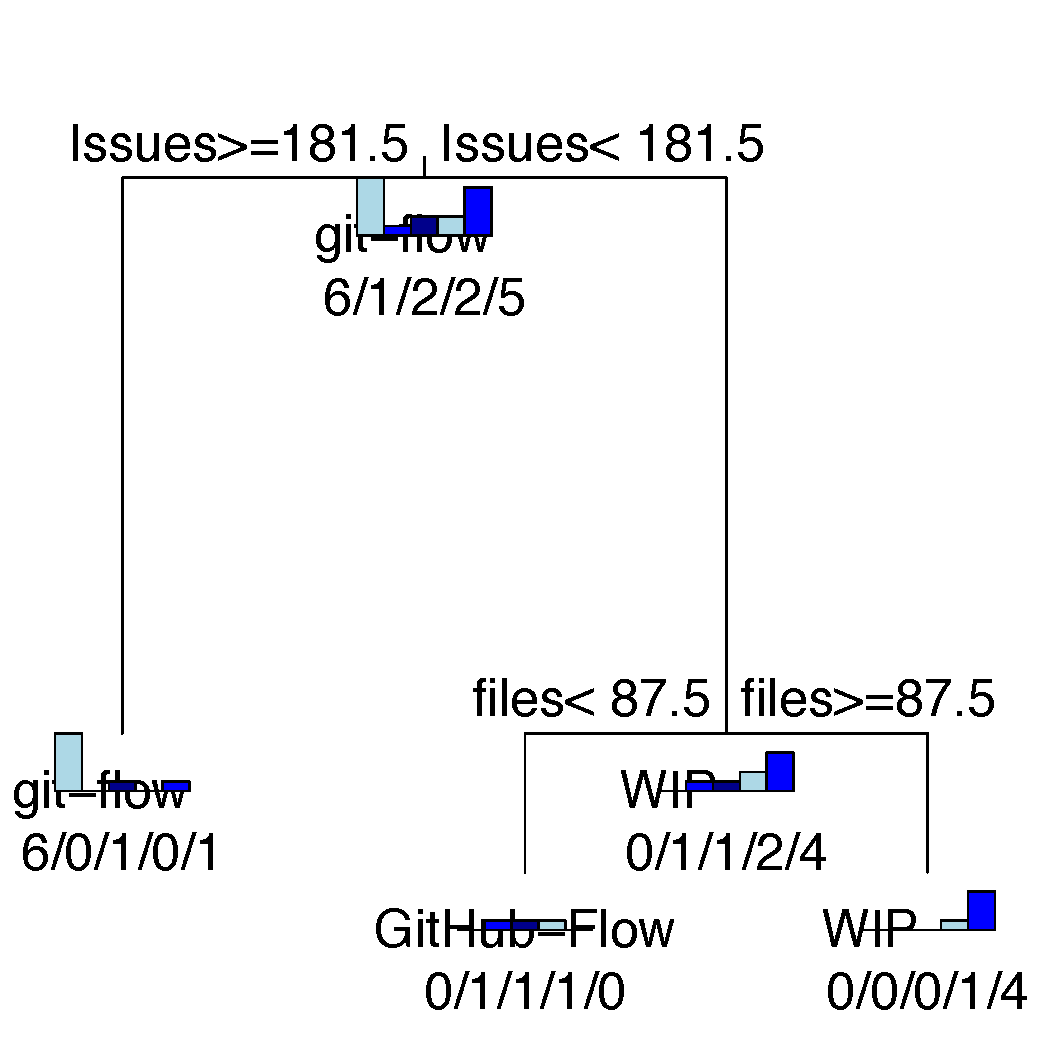
\includegraphics[width=45mm]{DecisionTree1.pdf}
   \caption{決定木1}
   \label{left}
  \end{center}
 \end{minipage}%
 \begin{minipage}{0.5\hsize}
  \begin{center}
   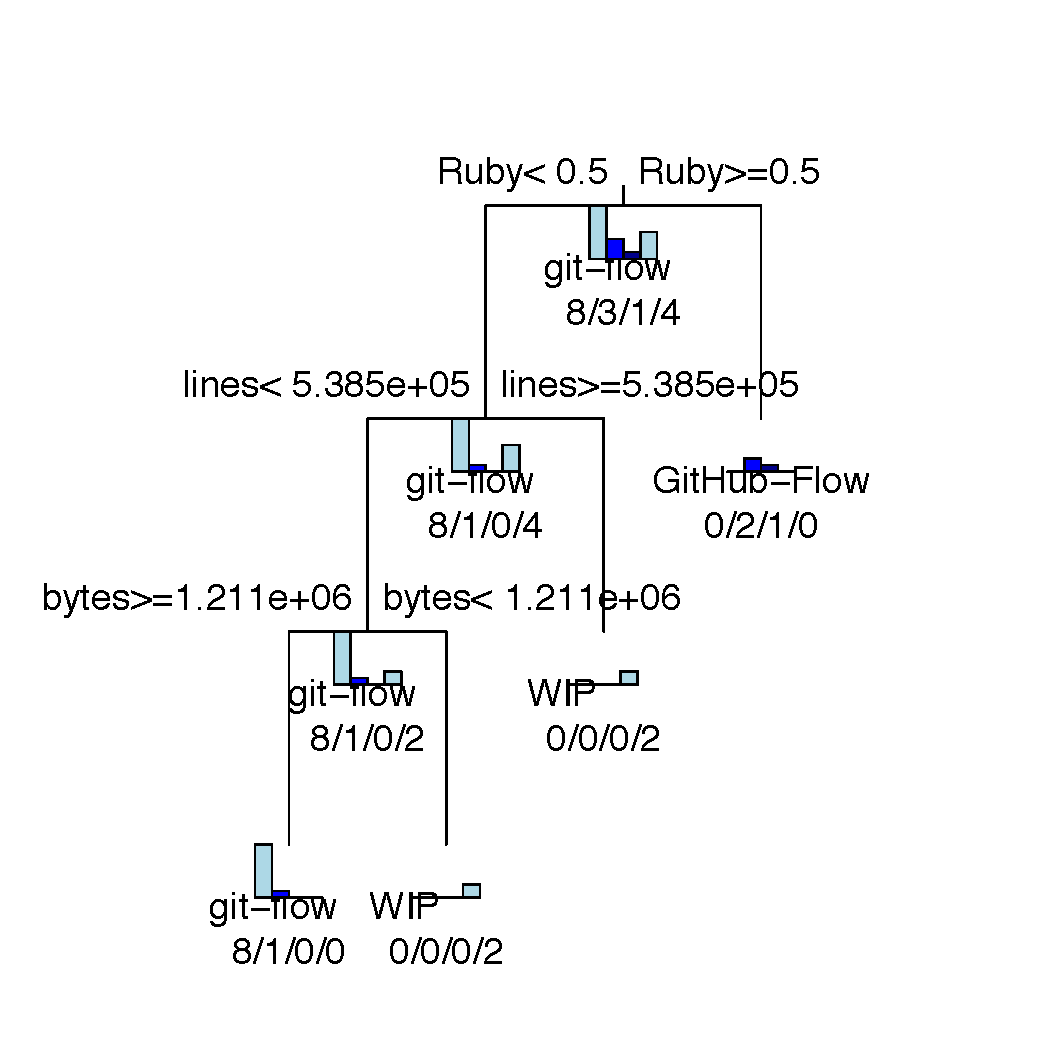
\includegraphics[width=45mm]{DecisionTree2.pdf}
   \caption{決定木2}
   \label{right}
  \end{center}
 \end{minipage}
\end{figure}


\section{今後の計画}

時系列データを分析に含めた場合,基準にどのような変化があるか調査する.そうすることで,開発スピードを含めた開発フローを選択する基準が求められる.


\bibliographystyle{junsrt}
\bibliography{biblio}%「biblio.bib」というファイルが必要.

\end{document}
